\documentclass[a4paper]{article}

\usepackage{fontspec}
\setmainfont[
    ItalicFont={Georgia-Italic},
]{Georgia}
\setsansfont[
	UprightFont={SF Pro Display-Medium},
	BoldFont={SF Pro Display-Bold}
]{SF Pro Display}

\usepackage{amsmath, amsthm, amssymb}
\usepackage{mathtools}
\usepackage[many]{tcolorbox}
\usepackage{xcolor}
\usepackage{titlesec}
\usepackage{titling}
\usepackage{enumitem}   


\definecolor{grey}{rgb}{0.5,0.5,0.5}
\definecolor{lightgrey}{rgb}{0.9,0.9,0.9}
\definecolor{darkgrey}{rgb}{0.3,0.3,0.3}
\definecolor{orange}{rgb}{0.94, 0.55, 0.294}
\definecolor{pink}{rgb}{0.94, 0.29, 0.7}
\definecolor{yellow}{rgb}{1, 0.749, 0}

\newcommand{\chapfnt}{\fontsize{16}{19}}
\newcommand{\secfnt}{\fontsize{18}{17}}
\newcommand{\ssecfnt}{\fontsize{14}{14}}
\renewcommand{\hline}{\noindent\makebox[\linewidth]{\rule{12cm}{1pt}}}
\newcommand{\vip}[1]{\textit{\textbf{#1}}}
\newcommand{\R}{\mathbb{R}} % Reelle Zahlen
\newcommand{\N}{\mathbb{N}} % Natürliche Zahlen
\newcommand{\Z}{\mathbb{Z}} % Ganze Zahlen
\newcommand{\C}{\mathbb{C}} % Komplexe Zahlen
\newcommand{\Q}{\mathbb{Q}} % Rationale Zahlen

\titleformat{\chapter}[display]
{\normalfont\chapfnt\bfseries}{\chaptertitlename\ \thechapter}{20pt}{\chapfnt}

\titleformat{\section}
{\normalfont\sffamily\secfnt\bfseries}{\thesection}{}{}

\titleformat{\subsection}
{\normalfont\sffamily\ssecfnt\mdseries}{\thesubsection}{}{}

\titleformat{\subsubsection}
{\normalfont\sffamily\ssecfnt\mdseries\color{grey}}{\thesubsection}{}{}

\titlespacing*{\chapter} {0pt}{50pt}{40pt}
\titlespacing*{\section} {0pt}{6pt}{8pt}
\titlespacing*{\subsection} {0pt}{12pt}{8pt}


\linespread{1.3}



%\usepackage{geometry}
%\setlength{\columnsep}{32mm}
%\geometry{
% left=22mm,
% right=22mm,
% bottom=32mm,
% top = 20mm
%}


\newtcbtheorem[auto counter,number within=section]{theorem}%
  {Theorem}{
  		fonttitle=\upshape, 
  		fontupper=\upshape,
  		boxrule=0pt,
  		leftrule=3pt,
  		arc=0pt,auto outer arc,
  		colback=white,
  		colframe=pink,
  		colbacktitle=white,
  		coltitle=pink,
  		oversize,
  		enlarge top by=1mm,
  		enlarge bottom by=1mm,
    	enhanced jigsaw,
    	interior hidden, 
    	before skip=12pt,
    	overlay={
    		\draw[line width=1.5pt,pink] (frame.north west) -- (frame.south west);
  		}, 
  		frame hidden}{theorem}
  		
\newtcbtheorem[]{issue}%
  {To prove}{
        theorem name,
  		fonttitle=\upshape, 
  		fontupper=\upshape,
  		boxrule=0pt,
  		leftrule=3pt,
  		arc=0pt,auto outer arc,
  		colback=white,
  		colframe=pink,
  		colbacktitle=white,
  		coltitle=pink,
  		oversize,
  		enlarge top by=1mm,
  		enlarge bottom by=1mm,
    	enhanced jigsaw,
    	interior hidden, 
    	before skip=12pt,
    	after skip=0pt,
    	overlay={
    		\draw[line width=1.5pt,pink] (frame.north west) -- (frame.south west);
  		}, 
  		frame hidden}{issue}

\newtcbtheorem[auto counter,number within=section]{lemma}%
  {Lemma}{
  		fonttitle=\upshape, 
  		fontupper=\upshape,
  		boxrule=1pt,
  		toprule=0pt,
  		leftrule=3pt,
  		arc=0pt,auto outer arc,
  		colback=white,
  		colframe=orange,
  		colbacktitle=white,
  		coltitle=orange,
  		oversize,
  		enlarge top by=1mm,
  		enlarge bottom by=1mm,
    	enhanced jigsaw,
    	interior hidden, 
    	before skip=12pt,
    	after skip=0pt,
    	overlay={
    		\draw[line width=1.5pt,orange] (frame.north west) -- (frame.south west);
  		}, 
  		frame hidden}{lemma}
  		
 \newtcbtheorem[auto counter,number within=section]{definition}%
  {Definition}{
  		fonttitle=\upshape, 
  		fontupper=\upshape,
  		boxrule=1pt,
  		toprule=0pt,
  		leftrule=3pt,
  		arc=0pt,auto outer arc,
  		colback=white,
  		colframe=orange,
  		colbacktitle=white,
  		coltitle=orange,
  		oversize,
  		enlarge top by=1mm,
  		enlarge bottom by=1mm,
    	enhanced jigsaw,
    	interior hidden, 
    	before skip=12pt,
    	overlay={
    		\draw[line width=1.5pt,orange] (frame.north west) -- (frame.south west);
  		}, 
  		frame hidden}{definition}
    	
\newtcbtheorem[auto counter,number within=section]{example}%
  {Beispiel}{
  		fonttitle=\upshape, 
  		fontupper=\upshape,
  		boxrule=0pt,
  		leftrule=3pt,
  		arc=0pt,auto outer arc,
  		colback=white,
  		colframe=grey,
  		colbacktitle=white,
  		coltitle=grey,
  		oversize,
  		enlarge top by=1mm,
  		enlarge bottom by=1mm,
    	enhanced jigsaw,
    	interior hidden, 
    	before skip=12pt,
    	overlay={
    		\draw[line width=1.5pt,grey] (frame.north west) -- (frame.south west);
  		}, 
  		frame hidden}{example}
    	
\newtcbtheorem[auto counter,number within=section]{note}%
  {Notiz}{
  		fonttitle=\upshape, 
  		fontupper=\upshape,
  		boxrule=0pt,
  		leftrule=3pt,
  		arc=0pt,auto outer arc,
  		colback=white,
  		colframe=yellow,
  		colbacktitle=white,
  		coltitle=yellow,
  		oversize,
  		enlarge top by=1mm,
  		enlarge bottom by=1mm,
    	enhanced jigsaw,
    	interior hidden, 
    	before skip=12pt,
    	overlay={
    		\draw[line width=1.5pt,yellow] (frame.north west) -- (frame.south west);
  		}, 
  		frame hidden}{note}
  		
\newtcbtheorem[]{important}%
  {Wichtig}{
  		fonttitle=\upshape, 
  		fontupper=\upshape,
  		boxrule=0pt,
  		leftrule=3pt,
  		arc=0pt,auto outer arc,
  		colback=white,
  		colframe=pink,
  		colbacktitle=white,
  		coltitle=pink,
  		oversize,
  		enlarge top by=1mm,
  		enlarge bottom by=1mm,
    	enhanced jigsaw,
    	interior hidden, 
    	before skip=12pt,
    	overlay={
    		\draw[line width=1.5pt,pink] (frame.north west) -- (frame.south west);
  		}, 
  		frame hidden}{important}
    	
\renewcommand{\baselinestretch}{1.4} 
\makeatletter
\let\old@rule\@rule
\def\@rule[#1]#2#3{\textcolor{lightgrey}{\old@rule[#1]{#2}{#3}}}
\makeatother

\begin{document}
 \noindent 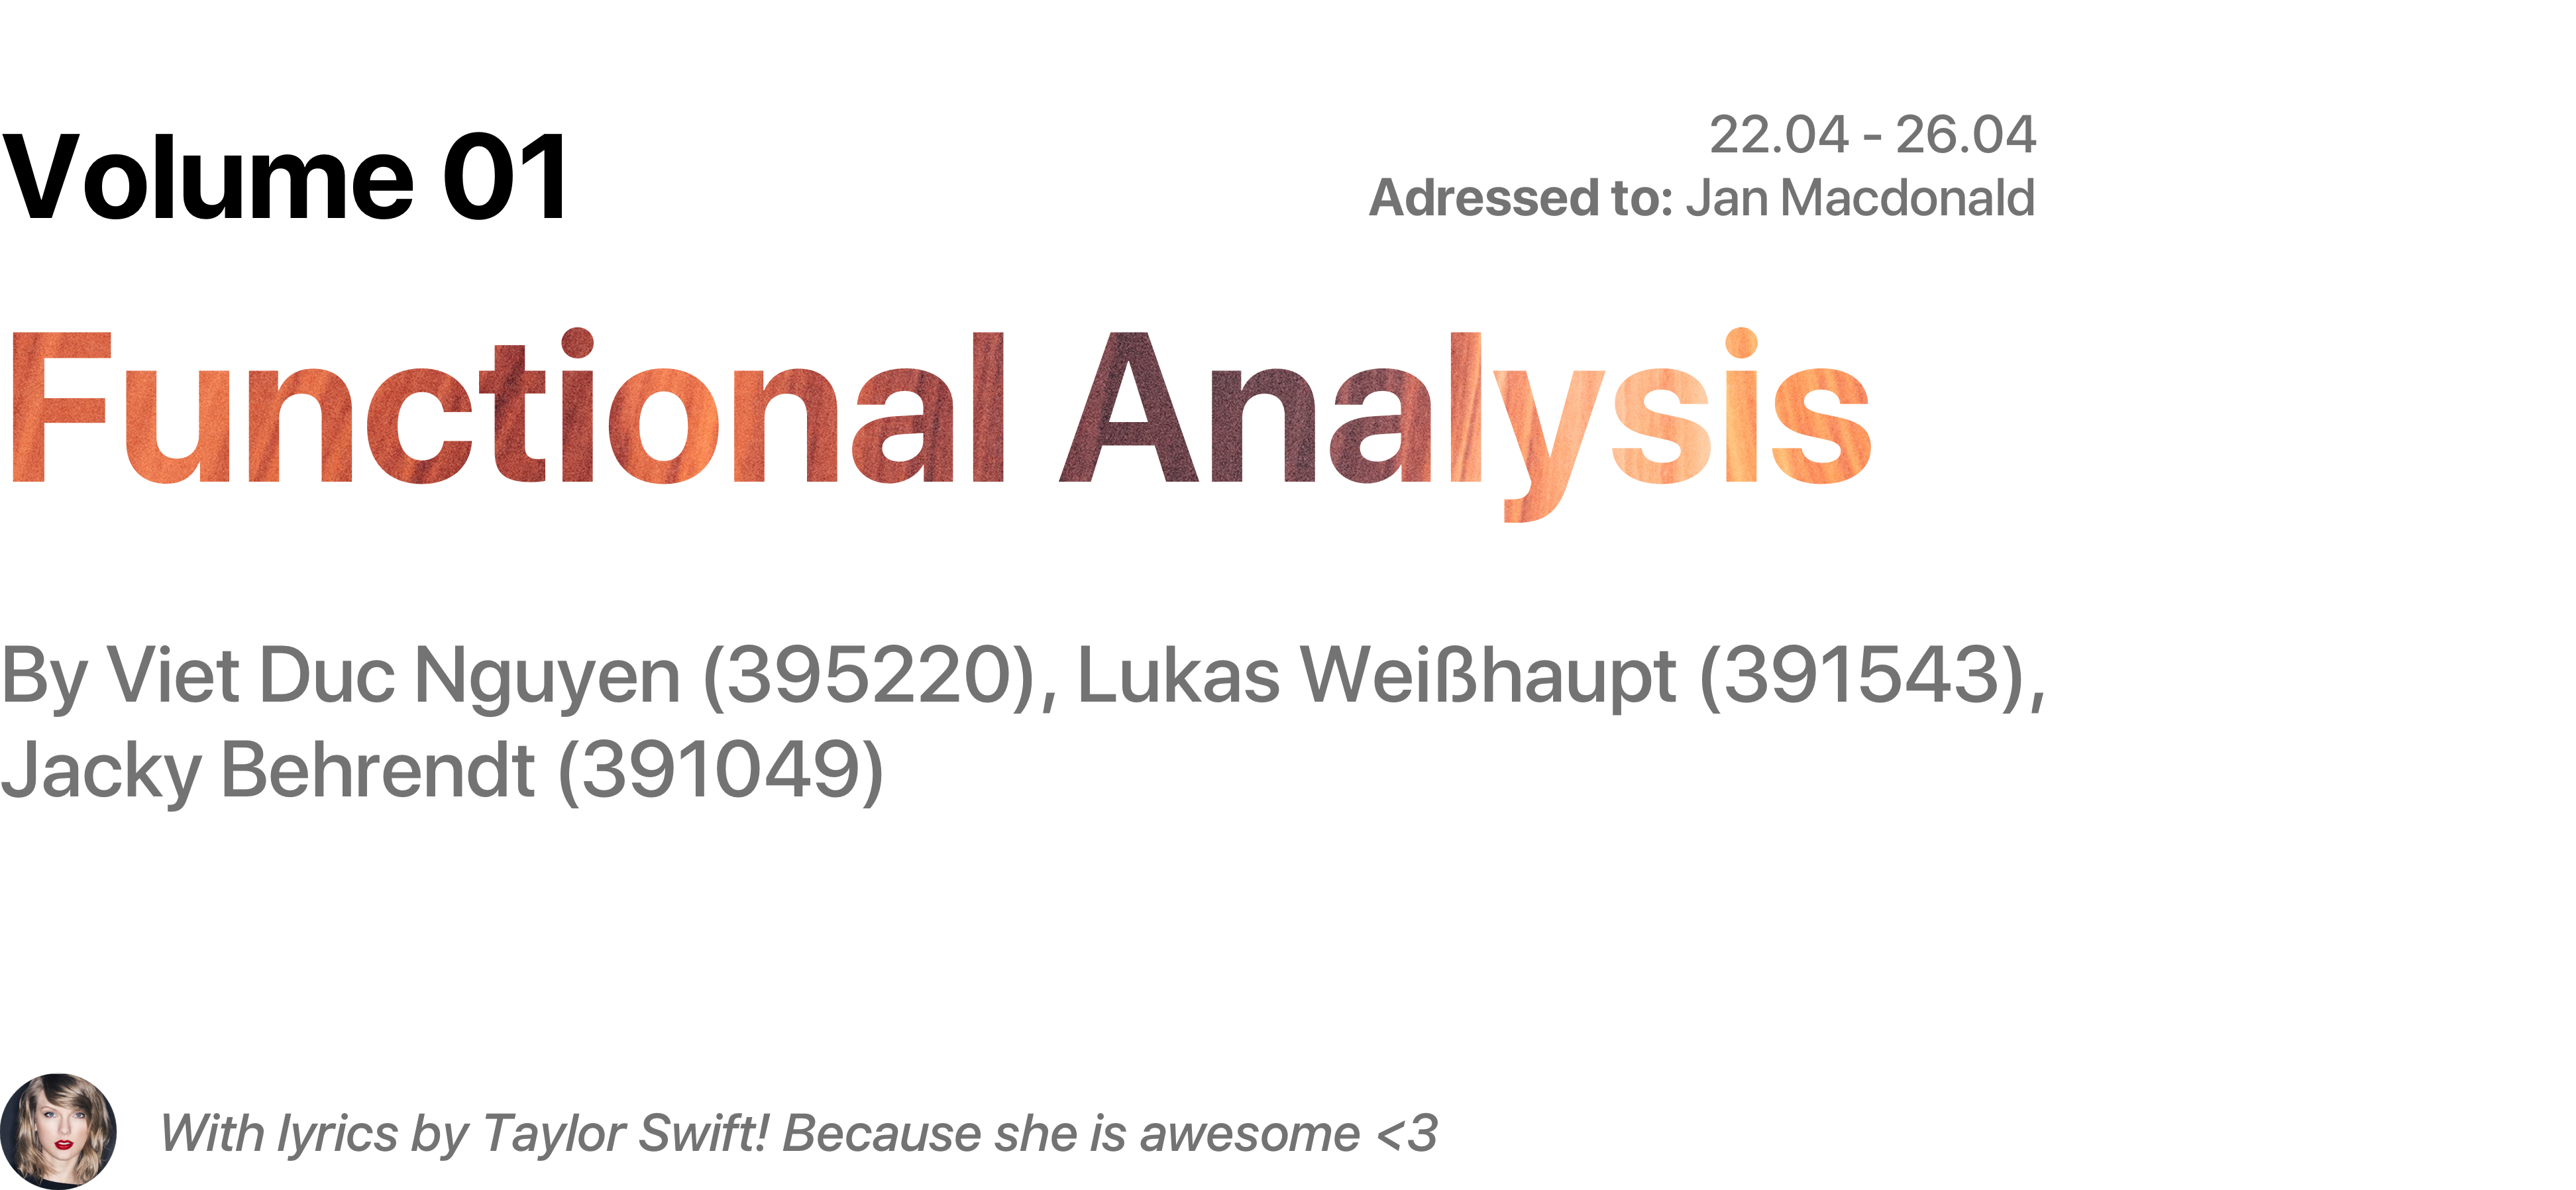
\includegraphics[width=17cm]{lol.png}

\hline

\subsection*{We love Taylor Swift}
\subsubsection*{I stay out too late, got nothin' in my brain\\ That's what people say, hmm, that's what people say, hmm}
{\color{grey}\emph{From her masterwork }\vip{Shake it Off}}

\hline 

\textbf{Rate us on Moses!} 

Help us improving our service. We believe in our zero tolerance policy toward unfinished and wrong solutions. Our quality testing ensures the best tutor experience possible. Every word is \vip{carefully} typed, and formulas are \vip{handcrafted} by top notch mathematicians with \vip{+2 years experience}. However, if you have got any criticisms, we would like to hear from you! Just drop a comment, and we will come back to you.

\hline

\newpage

\subsection*{Exercise 1}
{\color{grey}\emph{Written by Viet Duc Nguyen / Berlin, Germany / 23.04.2019, 09:30 AM}}

\begin{issue}{}{}
$(X,d_1) \text{ and } (X,d_2) \text{ are equivalent } \iff \text{ the convergent sequences concide}$
\end{issue}
\begin{proof}
$\implies$ Let $(X,d_1)$ and $(X,d_2)$ be equivalent metric spaces. Let $(x_n)_{n \in \mathbb N}$ be any convergent sequence in $(X,d_1)$, i.e. $x_n \to x \in X$ in $(X,d_1)$. 

\textbf{Goal:} We will show that $(x_n)_n$ converges in $(X,d_2)$, i.e. $x_n \to x$ in $(X,d_2)$.

Let $\epsilon > 0$. Due to the equivalence of $U_1$ and $U_2$, we find $r > 0$ such that $U_1(x,r) \subset U_2(x,\epsilon)$. Then, choose $N \in \mathbb N$ such that $x_n \in U_1(x, r)$ for all $n \geq N$; finding such $N$ is possible since $(x_n)_n$ is convergent in $(X,d)$ after the assumption. Thus, it follows that $x_n \in U_2(x, \epsilon)$ for all $n \geq N$. Per definition, $(x_n)_n$ converges in $(X,d_2)$. Same argument applies to show that $(x_n)_n$ converges in $(X,d_1)$ if  $(x_n)_n$ is convergent in $(X,d_2)$.

$\impliedby$ Assume that the convergent sequences in $(X,d_1)$ and $(X,d_2)$ are the same. We will prove the equivalence of the metric spaces by contradiction.

\textbf{Goal:} We will construct a sequence $(x_n)_n$ that converges in $(X,d_1)$ but not in $(X,d_2)$ if we assume that the metric spaces are \emph{not} equivalent. 

Let $(X,d_1)$ and $(X,d_2)$ be not equivalent. Hence, there is a $x\in X$ and $\epsilon > 0$ such that for all $r > 0$ it holds: $U_1(x,r) \not \subset U_2(x, \epsilon)$ or $U_2(x,r) \not \subset U_1(x, \epsilon)$. Consider the first case (the proof for the other case is identical). Thus, there exists $x_r$ for each $r > 0$ such that $d_1(x_r,x) < r$ and $d_2(x_r,x) \geq \epsilon$. Construct the sequence $(y_n)_n$ with $y_n \coloneqq x_{\frac{1}{n}}$. Finally, $y_n \to x$ in $(X,d_1)$ but $y_n \not \to x$ in $(X,d_2)$. Contradiction, for the sequences in both metric spaces conincide per assumption. The metric spaces must be therefore equivalent.
\end{proof}

\hline


\begin{issue}{}{}
Show that $\delta(x,y) = \frac{d(x,y)}{1+d(x,y)}$ is a metric for a metric space $(X,d)$.
\end{issue}

\begin{proof}
Let $x,y,z \in X$. $\delta$ is zero if and only if the numerator is zero. The numerator is $d(x,y)$; thus, $\delta(x,y) = 0 \iff d(x,y) = 0 \iff x = y$. The \vip{symmetry} follows from the {symmetry} of $d$. Observe that $\delta(x,y) = \frac{d(x,y)}{1+d(x,y)} = \frac{d(y,x)}{1+d(y,x)} = \delta(y,x)$. Concerning the \vip{triangle inequality}: 
\begin{align*}
    \delta(x,z) \leq \frac{d(x,z)}{1+d(x,z)} \overset{(*)}{\leq} \frac{d(x,y) + d(y,z)}{1+d(x,y) + d(y,z)} &\leq \frac{d(x,y)}{1+d(x,y)} + \frac{d(y,z)}{1 + d(y,z)} \\
    &= \delta(x,y) + \delta(y,z),
\end{align*}
where $(*)$ follows from the monotony of $x \mapsto \frac{x}{1+x}$ (remains to be shown). $\delta$ is therefore a norm.
\end{proof}

\hline

\begin{lemma}{}{}
$f(x) = \frac{x}{1+x}$ is monotonically increasing.
\end{lemma}

\begin{proof}
The derivative reads $\frac{1}{(1+x)^2}$. Since the derivative is strictly positive and $f$ is continuous, $f$ is monotonically increasing.
\end{proof}

\hline

\begin{issue}{}{}
Show that $(X,d)$ and $(X,\delta)$ are equivalent metric spaces.
\end{issue}

\begin{proof}
To show the claim we prove that the convergent sequences coincide. Let $(x_n)_n$ be a convergent sequence in $(X,d)$ with limit $x \in X$. The convergence of $(x_n)_n$ in $(X, \delta)$ follows from $\delta(x,y) = \frac{d(x,y)}{\underbrace{1+d(x,y)}_{\geq 1}} \leq d(x,y)$ for all $x,y \in X$. Thus, for any $\epsilon > 0$ we will find a number $N \in \mathbb N$ (due to the convergence of $(x_n)_n$ in $(X,d)$) such that 
\[
	\forall n \geq N: \delta(x_n,x) \leq d(x_n,y) < \epsilon,
\]
which implies the convergence of $(x_n)_n$ in $(X, \delta)$.

Consider a convergent sequence $(x_n)_n$ in $(X,\delta)$ with limit $x \in X$. We want to prove that $(x_n)_n$ also converges to the same limit $x$ in $(X,d)$. Again, take any arbitrary positive $\epsilon$, and we need to find a number $N \in \mathbb N$ such that $d(x_n,x) < \epsilon$ for all $n \geq N$. 

Define $f: X \to \mathbb R, u \mapsto \frac{u}{1+u}$. This function is continuous \emph{(make sure this is clear to you!!!!!!)}, and injective (due to the strict monotonicity as stated in the previous lemma). We know that $f(d(x_n,x)) \to 0$ from the convergence of $(x_n)_n$ in $(X,\delta)$. Observe that $f(u) = 0 \iff u = 0$. By injectivity and monotonicity of $f$, we deduct
\[
	f(u_n) \to 0 \implies u_n \to 0, \quad \forall (u_n)_n \subset X.
\]
Thus, $d(x_n,x) \to 0$ impliying the convergence of $(x_n)_n$ in $(X,d)$.
\end{proof}

\hline

\subsection*{We love Taylor Swift}
\subsubsection*{"I'm sorry, the old Taylor can't come to the phone right now"\\
"Why?"\\
"Oh, 'cause she's dead!"}
{\color{grey}\emph{From her masterwork }\vip{Look what you made me do}}

\hline 

\subsection*{Aufgabe 2}
Let $X, d_1$ and $d_2$ be as specified. We want to show that $d_2$-open sets are $d_1$-open and vice versa.

Let $A$ be $d_2$-open and $x \in A$. Then there is an $\epsilon > 0$ with $U_2(x,\epsilon)\subset A$. Now let $y\in U_1(x,\epsilon)$. We obtain
\begin{align*}
    \epsilon &> d_1(x,y) = |\frac{1}{x}-\frac{1}{y}| = \frac{|x-y|}{|xy|}\\
    &\implies |x-y|<\epsilon xy < \epsilon\\
    &\implies y\in U_2(x,\epsilon)\subset A
\end{align*}
Which shows that $A$ is also $d_1$-open.

For the second step, suppose that $A$ is $d_1$-open. For each point $a\in A$ we want to find an open $\epsilon$-Ball that is a subset of $A$.

Let $a\in A$ and let $\epsilon$ be so that $U_1(a,\epsilon) \subset A$ and $\epsilon\leq 1$. Now define $\epsilon' := \frac{a^2 \epsilon}{2}$ and let $x\in U_2(a,\epsilon')$. Notice that $\epsilon'\leq \frac{a}{2}$ which means $x>\frac{a}{2}$ for any $x\in U_2(a,\epsilon')$. Now we have:
\begin{align*}
    d_2(a,x)<\epsilon' \implies |a-x|<\epsilon' \implies \frac{|a-x|}{ax}<\frac{\epsilon'}{ax} \implies |\frac{1}{a}-\frac{1}{x}|<\frac{2\epsilon'}{a^2}
\end{align*}
Thus, $d_1(a,x) < \epsilon$ and furthermore $x\in A$.

Now regarding completeness:

The metric space $(x,d_2)$ is obviously not complete as the sequence $(\frac{1}{n})_{n\in\mathbb N}$ is a Cauchy-sequence but not convergent in $(0,1]$.

On the other hand, we can show that all $d_1$-Cauchy-sequences are $d_2$-Cauchy-sequences:

Let $(x_n)_{n\in\mathbb N}$ be a $d_1$-Cauchy-sequence. That means $\forall \epsilon\! >\! 0\ \exists N\!\in\!\mathbb N \ \forall k,l>N: |\frac{1}{x_k}-\frac{1}{x_l}|<\epsilon$ which implies $|x_k-x_l|<\epsilon x_kx_l < \epsilon$.

Now since we know that in $([0,1],d_2)$ all Cauchy-sequences converge it is sufficient to show that any sequence $(x_n)_{n\in\mathbb N}\subset (0,1]$  which converges to zero - in $([0,1],d_2)$ - is not a Cauchy-sequence in $((0,1],d_1)$. You can see that as follows: 

Since $x_n \longrightarrow 0$ for $n\to\infty$ we know that for all $\epsilon > 0$ there is an index $N\in \mathbb N$ so that for all $k>N$: $x_k<\epsilon$. Now set $\epsilon = 1$ and let $N\in\mathbb N$ be arbitrary. Then, find another arbitrary $k>N$ with $\frac{1}{x_k} := \delta$. For this $\delta > 0$ we can find an $l>N$ with $|\frac{1}{x_l}|>\delta+1$. Thus $|\frac{1}{x_k} - \frac{1}{x_l}|>1$ and $(x_n)_{n\in\mathbb N}$ is not a Cauchy-sequence in $((0,1],d_1)$.

All other Cauchy-sequences in $((0,1],d_2)$ are convergent because they are Cauchy-sequences in $([0,1],d_2)$ whose limit is not 0 but somewhere in $(0,1]$ and thus in $((0,1],d_2)$. This means that all Cauchy-sequences in $((0,1],d_1)$ are also convergent. \qed

\hline

\subsection*{We love Taylor Swift}
\subsubsection*{Nice to meet you, where you been?\\
I could show you incredible things}
{\color{grey}\emph{From her masterwork }\vip{Blank Space}}

\hline 

\subsection*{Aufgabe 3}
Let $\mathcal{S}$ be the space of $all$ sequences $(x_i)_{i = 1}^{\infty}$ of complex numbers. Verify that 
\begin{equation*}
    d(x,y) := \sum_{i = 1}^{\infty} \frac{2^{-i} |x_i - y_i|}{1+ |x_i - y_i|}, \quad x,y \in \mathcal{S}
\end{equation*}
provides a metric on the space $S$. Show that a sequence $(x^{(n)})_{n \in \N} \subset \mathcal{S}$ converges to $x \in \mathcal{S}$ in $(\mathcal{S}, d)$ if and only if $x_i^{(n)} \to x_i$ for all $i \in \N$. Prove that $\mathcal{S}$ is complete.
\begin{lemma}{}{}
    d(x,y) provides a metric 
\end{lemma}
\begin{proof}
Let $x,y \in \mathcal{S}$.
Since for $x \in \R$ it holds that $\frac{x}{1+x} \leq 1$ we see:
\begin{align*}
    d(x,y) = \sum_{i = 1}^{\infty} \frac{2^{-i} |x_i - y_i|}{1+ |x_i - y_i|} \leq \sum_{i = 1}^{\infty} 2^{-i} = 1 
\end{align*}
This shows that $d: \mathcal{S} \times \mathcal{S} \mapsto \R $.
We will now demonstrate that $d$ satisfies the conditions for a metric as defined in Definition 1.1. Let $x,y,z \in \mathcal{S}$. 
\begin{enumerate}
        \item $d(x,y) = 0 \Leftrightarrow x = y$\\
        $"\Rightarrow"$ Let $d(x,y) = 0$. This results in $ \sum_{i = 1}^{\infty} \frac{2^{-i} |x_i - y_i|}{1+ |x_i - y_i|} = 0 $ 
        Since all summands of this sum are positive, all of them have to be zero for the sum to be zero. This implies for $i \in \N$
        \begin{align*}
            0 = \frac{2^{-i} |x_i - y_i|}{1+ |x_i - y_i|}
            \Rightarrow 0= |x_i - y_i| \Rightarrow x_i = y_i
        \end{align*}
        For $i \in \N$ we see  $x_i = y_i $ and therefor $x = y$.\\
        $"\Leftarrow"$ Let $x = y $. So for $i \in \N$ $x_i = y_i$ and $|x_i -y_i| = 0 $. For $d$ this results in: 
        \begin{align*}
            0 = \sum_{i = 1}^{\infty} \frac{2^{-i} |x_i - y_i|}{1+ |x_i - y_i|} = d(x,y)
        \end{align*}
        \item $d(x,y) = d(y,x)$
        \begin{align*}
            d(x,y) = \sum_{i = 1}^{\infty} \frac{2^{-i} |x_i - y_i|}{1+ |x_i - y_i|} = \sum_{i = 1}^{\infty} \frac{2^{-i} |(-1)(y_i - x_i)|}{1+ |(-1)(y_i - x_i)|} = \sum_{i = 1}^{\infty} \frac{2^{-i} |y_i - x_i|}{1+ |y_i - x_i|} = d(y,x)
        \end{align*}
        \item $d(x,y) \leq d(x,z) + d(z,y)$
        To show the triangle inequality we will use that the function $t \mapsto t/1+ t$ is monotonically increasing on $(0,\infty)$. We have already shown this in Exercise 1. 
        \begin{align*}
            d(x,y) & = \sum_{i = 1}^{\infty} \frac{2^{-i} |x_i - y_i|}{1+ |x_i - y_i|} \\
            & \leq \sum_{i = 1}^{\infty} \frac{2^{-i} (|x_i - z_i| + |z_i - y_i|)}{1+ |x_i - z_i| + |z_i - y_i|}\\
            &= \sum_{i = 1}^{\infty} \frac{2^{-i} |x_i - z_i|}{1+ |x_i - z_i| + |z_i - y_i|}  + \frac{2^{-i} |z_i - y_i|}{1+ |x_i - z_i| + |z_i - y_i|}\\
            & \leq \sum_{i = 1}^{\infty} \frac{2^{-i} |x_i - z_i|}{1+ |x_i - z_i|}  + \frac{2^{-i} |z_i - y_i|}{1 + |z_i - y_i|}\\
            & = \sum_{i = 1}^{\infty} \frac{2^{-i} |x_i - z_i|}{1+ |x_i - z_i|}  + \sum_{i = 1}^{\infty} \frac{2^{-i} |z_i - y_i|}{1 + |z_i - y_i|}\\
            & = d(x,z) + d(z,y)
        \end{align*}

\end{enumerate}
\end{proof}
\begin{issue}{}{}
    $(x^{(n)}) \subset \mathcal{S}$ converges to $x \in \mathcal{S}$ in $(\mathcal{S},d)$ if and only if $x_i^{(n)} \to x_i$ for all $i \in \N$
\end{issue}
\begin{proof}
$"\Rightarrow"$ Let $(x^{(n)}) \subset \mathcal{S}$ and $(x^{(n)})$ converges to $x \in \mathcal{S}$ in $(\mathcal{S},d)$.
Towards a contradiction we assume that there is $i \in \N$, such that $x_i^{(n)} \nrightarrow x_i$. We can then find $\delta > 0$ such that for every $N \in \N$ there is a $n \geq N$ with $|x_i - x_i^{(n)}|> \delta$. We choose $\varepsilon \leq \frac{2^{-i} \delta}{1+ \delta}$:
\begin{align*}
    \varepsilon \leq \frac{2^{-i} \delta}{1+ \delta} \leq \sum_{i = 1}^{\infty} \frac{2^{-i} |x_i -  x_i^{(n)}|}{1+ |x_i -  x_i^{(n)}|} = d(x, x^{(n)})
\end{align*}
which would be a contradiction of $(x^{(n)})$ converging to x.\\\\
$"\Leftarrow"$ For $i \in \N$ $x_i^{(n)} \to x_i$. Let $\Tilde{\varepsilon} > 0 $. We choose $m \in \N$ such that $\Tilde{\varepsilon} > (\frac{1}{2})^{(m-1)}$. Let $\varepsilon = (\frac{1}{2})^{(m)}$. Since for $i \in \N$ $x_i^{(n)} \to x_i$ we can find for $i \in \{1,...,m\}$ $N_{\varepsilon,i} \in \N$ such that for $n \geq N_{\varepsilon,i}$ $|x_i- x_i^{(n)}|  < \varepsilon$. Set $N = \max\{N_{\varepsilon,1},...,N_{\varepsilon,m} \}$. For $n \geq N$ we obtain: 
\begin{align*}
    d(x, x^{(n)}) & = \sum_{i = 1}^{\infty} \frac{2^{-i} |x_i -  x_i^{(n)}|}{1+ |x_i -  x_i^{(n)}|}\\
    & \leq \sum_{i = 1}^{m} \frac{2^{-i} \varepsilon}{ 1+ \varepsilon } + \sum_{i = m+1}^{\infty} \frac{2^{-i} |x_i -  x_i^{(n)}|}{1+ |x_i -  x_i^{(n)}|}\\
    & \leq \sum_{i = 1}^{m} 2^{-i} \varepsilon + \sum_{i = m+1}^{\infty} 2^{-i} \\
    & \leq (\frac{1}{2})^m + (\frac{1}{2})^m \\
    & = 2 (\frac{1}{2})^m \\
    & = (\frac{1}{2})^{m-1} \\
    & < \Tilde{\varepsilon}
\end{align*}
Hence $(x^{(n)}) \subset \mathcal{S}$ converges to $x \in \mathcal{S}$.\\\\
\end{proof}
In order to prove that $(\mathcal{S}, d )$ is complete we will first prove the following lemma:
\begin{lemma}{}{}
    Let $d_1(x,y) = \frac{|x-y|}{1+|x-y|}$ and $d_2(x,y) = |x-y|$. A Cauchy-sequence in $(X, d_1)$ is also a Cauchy-sequence in $(X, d_2)$. 
\end{lemma}
\begin{proof}
Let $(x_n)_{n \in \N}$ be a $d_1$-Cauchy-sequence.
In the first exercise we proofed that $d_1$ and $d_2$ are equivalent.
Due to the equivalence of $d_1$ and $d_2$ for  every $\varepsilon > 0$ exists $\delta > 0$ such that $U(d_1, \delta) \subset U(d_2, \varepsilon)$.
Since $(x_n)_{n \in \N}$ is a $d_1$-Cauchy-sequence for $\delta > 0$ exists  $N_{\delta} \in \N$ such that for all $n,m \geq N_{\delta}$ $d_1(x_n,x_m) < \delta$. With the inclusion $U(d_1, \delta) \subset U(d_2, \varepsilon)$ then follows:
\begin{align*}
    d_1(x_n,x_m) < \delta \Rightarrow d_2(x_n, x_m) < \varepsilon 
\end{align*}
Therefor $(x_n)_{n \in \N}$ is a $d_2$-Cauchy-sequence .
\end{proof}
\begin{issue}{}{}
    $(\mathcal{S}, d )$ is complete
\end{issue}
\begin{proof}
 Let $(x^{(n)})_{n \in \N}$ be a Cauchy-Sequence in $\mathcal{S}$.
Since $(x^{(n)})_{n \in \N}$ is a Cauchy-Sequence, for every $\varepsilon > 0$ exists $N_{\varepsilon} \in \N$ such that for $n,m \geq N_{\varepsilon}$ $\varepsilon > d(x_n,x_m) $. From the definition of $d$ then follows for $i \in \N$: 
\begin{align*}
    & \varepsilon > d(x_n,x_m) = \sum_{i = 1}^{\infty} \frac{2^{-i} |x_i^{(m)} -  x_i^{(n)}|}{1+ |x_i^{(m)} -  x_i^{(n)}|} \\
    & \Rightarrow \varepsilon > \frac{2^{-i} |x_i^{(m)} -  x_i^{(n)}|}{1+ |x_i^{(m)} -  x_i^{(n)}|} \Rightarrow \varepsilon 2^{i} > \frac{|x_i^{(m)} -  x_i^{(n)}|}{1+ |x_i^{(m)} -  x_i^{(n)}|}
\end{align*}
Hence for $i \in \N$ the sequence $(x_i^{(n)})_{n \in \N}$ is also a Cauchy-Sequence in $(\C, \Tilde{d})$ with $\Tilde{d}(x,y): = \frac{|x-y|}{1 + |x-y|} $. 
From the first part of this exercise we already know that for a convergent sequence in $\mathcal{S}$ $x^{(n)} \to x$ is equivalent to $x_i^{(n)} \to x_i$ for all $i \in \N$. So if we show that for $i \in \N$ the Cauchy-sequence $(x_i^{(n)})_{n \in \N}$ converges to $x_i \in \C$ the Sequence $(x^{(n)})_{n \in \N}$ would also converge. Let $\Dot{d}(x,y) = |x-y|$.
From the previous Lemma we obtain that  $(x_i^{(n)})_{n \in \N}$ is a Cauchy-Sequence in $(\C, \Dot{d})$ and from Analysis 2 we know, that $(\C, \Dot{d})$ is complete. So the sequence $(x_i^{(n)})_{n \in \N}$ converges in $(\C, \Dot{d})$ and there exists a $x_i \in \C$, such that 
\begin{align*}
    \lim_{n \to \infty} x_i^{(n)} = x_i
\end{align*}
With the continuity of $f: t \mapsto \frac{t}{1+t}$, which we already stated in exercise 1 then follows: 
\begin{align*}
    \lim_{n \to \infty} \Dot{d}(x_i,x_i^{(n)}) = 0
    \Rightarrow \lim_{n \to \infty} \Tilde{d}(x_i,x_i^{(n)}) = \lim_{n \to \infty } \frac{\Dot{d}(x_i,x_i^{(n)})}{1+ \Dot{d}(x_i,x_i^{(n)})} = 
    \lim_{n \to \infty } f(\Dot{d}(x_i,x_i^{(n)})) = 0 
\end{align*}
So $x_i$ is the limit of $(x_i^{(n)})_{n \in \N}$ in $(\C, \Tilde{d})$. For $i \in \N$ we have shown that $x_i^{(n)} \to x_i$, which is equivalent to $(x^{(n)})$ converging in $\mathcal{S}$. Definition 1.3 implies then that $(\mathcal{S},d) $ is complete.\\
\end{proof}
\hline

\subsection*{We love Taylor Swift}
\subsubsection*{It seems like one of those nights\\
This place is too crowded, too many cool kids uh uh, uh uh}
{\color{grey}\emph{From her masterwork }\vip{22}}

\hline 

\subsection*{Aufgabe 4}

Let $1\leq p< q< \infty$. For $q=\infty$ not much is to be done as all sequences with finite sum have to be bounded. Now let $x = (x_n)_{n\in\mathbb N}\in \ell_p$ and define $A:=\{n\in\mathbb N: x_n>1\}$ and $B:=\{n\in\mathbb N: x_n\leq 1\}$. Then:
\begin{align*}
    \sum_{n\in\mathbb N} |x_n|^q = \sum_{n\in A} |x_n|^q + \sum_{n\in B} |x_n|^q
\end{align*}
where the first sum is finite because A has to be finite, otherwise the sequence could not be in $\ell_p$. But we also now have
\begin{align*}
    \sum_{n\in B} |x_n|^q \leq \sum_{n\in B} |x_n|^p < \sum_{n\in \mathbb N} |x_n|^q < \infty
\end{align*}
Thus, $\sum_{n\in \mathbb N} |x_n|^q$ is the sum of two finite terms and therefore it is finite itself.

There are $x\in\ell_q$ with $x\not \in \ell_p$: For all $n\in\mathbb N$, let \begin{align*}x_n := \Big(\frac{1}{n}\Big)^{\frac{1}{p}}.\end{align*}
For $q>p$ we obtain 
\begin{align*}
    \sum_{n\in\mathbb N} |\Big(\frac{1}{n}\Big)^{\frac{1}{p}}|^q = 
    \sum_{n\in\mathbb N} |\Big(\frac{1}{n}\Big)^{\frac{q}{p}}|<\infty
\end{align*}
because $\frac{q}{p}>1$ but
\begin{align*}
    \sum_{n\in\mathbb N} |\Big(\frac{1}{n}\Big)^{\frac{1}{p}}|^p = 
    \sum_{n\in\mathbb N} |\frac{1}{n}| = \infty.
\end{align*}
So we have found a sequence which is in $\ell_q$ but not in $\ell_p$.

\hline 

\section*{A final note}
\subsection*{We would like to thank everyone who has supported us over the years. A big thank you to \vip{you}! Without your awesome tutorials this would not have been possible.}
\subsubsection*{Stay tuned for next week's volume.}

\emph{In love,} \emph{Duc, Jacky \& Lukas.}
\end{document}